\section*{Problem Sheet 2:}
\label{sec:ps2}
\newcounter{psTwoQuestions}
\setcounter{psTwoQuestions}{0}
\renewcommand{\NewQuestion}[1]{\stepcounter{psTwoQuestions}\subsection*{Exercise \arabic{psTwoQuestions}: #1}}

\NewQuestion{This question is about the solutions to the Dirac equation}
By inserting into the Dirac equation and noting that these solutions do not depend on position but only on time (particle at rest). Show that the expressions below: 
\[\psi^{1}=e^{-imt}\vIV{1}{0}{0}{0}, \psi^{2}=e^{-imt}\vIV{0}{1}{0}{0}\]
\[\psi^{3}=e^{imt}\vIV{0}{0}{1}{0}, \psi^{4}=e^{imt}\vIV{0}{0}{0}{1}\]
are solutions to the Dirac equation. What is the interpretation of these states?
\answerbox{Insert $\psi^{1}$ to $\psi^{4}$ into the Dirac
  equation. Remember that since there is no spatial dependence
  $\vec{\nabla}\psi=0$. Remember the $m\psi$ term is
implicitly multiplied by $\underline{I}$. So that leaves:
\[ m\gamma^{0}\vIV{1}{0}{0}{0} -m\vIV{1}{0}{0}{0} = 0 \rightarrow m\vIV{1}{0}{0}{0}
-m\vIV{1}{0}{0}{0} =0,\]
\[ m\gamma^{0}\vIV{0}{1}{0}{0} -m\vIV{0}{1}{0}{0} = 0 \rightarrow m\vIV{0}{1}{0}{0}
-m\vIV{0}{1}{0}{0} =0,\]... similarly for the other solutions.\\
$\psi^{1}$: particle spin-up, $\psi^{2}$: particle spin-down
, $\psi^{3}$: anti-particle spin-up
, $\psi^{4}$: anti-particle spin-down
}



\NewQuestion{This question is about Pauli matrix manipulation}
Show that the spin operator $S^2\equiv \hat{\Sigma}_{x}^{\dagger}\hat{\Sigma}_{x}+ \hat{\Sigma}_{y}^{\dagger}\hat{\Sigma}_{y}+\hat{\Sigma}_{z}^{\dagger}\hat{\Sigma}_{z}$, is given by 
\[
\hat{S}^2=3/4 I_{4x4}
\]
where $I_{4x4}$ is the 4x4 unit matrix, $\hat{\Sigma}_{x}=1/2\mII{\sigma_{1}}{0}{0}{\sigma_{1}}$, 
$\hat{\Sigma}_{y}=1/2\mII{\sigma_{2}}{0}{0}{\sigma_{2}}$, 
$\hat{\Sigma}_{z}=1/2\mII{\sigma_{3}}{0}{0}{\sigma_{3}}$, 


and we used the relation $\sigma_{i}^{\dagger}\sigma_{i}=I_{2x2}$.
\answerbox{
Since $\hat{\vec{\Sigma}}$ operators are block diagonal
\[\hat{\Sigma}^{\dagger}\hat{\Sigma} =
\hat{\Sigma}_x^{\dagger}\hat{\Sigma}_x+
\hat{\Sigma}_y^{\dagger}\hat{\Sigma}_y+
\hat{\Sigma}_z^{\dagger}\hat{\Sigma}_z. 
\] Therefore
\[
\hat{\Sigma}^{\dagger}\hat{\Sigma}=1/4\left[\mII{\sigma_{1}^\dagger}{\underline{0}}{\underline{0}}{\sigma_{1}^\dagger}\mII{\sigma_{1}}{\underline{0}}{\underline{0}}{\sigma_{1}}+
\mII{\sigma_{2}^\dagger}{\underline{0}}{\underline{0}}{\sigma_{2}^\dagger}\mII{\sigma_{2}}{\underline{0}}{\underline{0}}{\sigma_{2}}+\\
\mII{\sigma_{3}^\dagger}{\underline{0}}{\underline{0}}{\sigma_{3}^\dagger}\mII{\sigma_{3}}{\underline{0}}{\underline{0}}{\sigma_{3}}\right]
\]
Now  can either expand the matrices or perform the block-diagonal
multiplication and invoke the properties of Pauli matrices to show
that
\[
\hat{\Sigma}^{\dagger}\hat{\Sigma}=3/4\mII{\underline{I}}{\underline{0}}{\underline{0}}{\underline{I}}
\]
}

\NewQuestion{This question is about the solutions to the Dirac equation and spin operators}
The general solutions to the Dirac equation for a particle, are given by
\[\psi^{1}(\vec{r},t)=\sqrt{|E|+m}  e^{-i(Et-\vec{p}\cdot\vec{r})}
\vIV{1}{0}{\frac{p_z}{(E+m)}}{\frac{p_x+ip_y}{E+m}},
\psi^{2}(\vec{r},t)=\sqrt{|E|+m}
e^{-i(Et-\vec{p}\cdot\vec{r})}\vIV{0}{1}{\frac{p_x-ip_y}{(E+m)}}{\frac{-p_z}{E+m}},
\]
By considering a particle moving only in the $z$-direction, how that $\psi^{1}$and $\psi^{2}$ are eigenstates of $\hat{\Sigma}_{z}$
\answerbox{
For particle moving along $z$, $p_x=p_y=0$. Therefore solutions become
\[
\psi^{1}(\vec{r},t)=\sqrt{|E|+m}  e^{-i(Et-p_zz)}
\vIV{1}{0}{\frac{p_z}{(E+m)}}{0},
\psi^{2}(\vec{r},t)=\sqrt{|E|+m}
e^{-i(Et-p_zz)}\vIV{0}{1}{0}{\frac{-p_z}{E+m}}
\]

So, multiplying each solution by $\hat{\Sigma}_z$ we have
\[
\hat{\Sigma}_z \psi^1 =
1/2\mII{\sigma_{3}}{\underline{0}}{\underline{0}} {\sigma_{3}} \psi^1 =1/2
\sqrt{|E|+m}
e^{-i(Et-\vec{p}\cdot\vec{r})}\vIV{1}{0}{\frac{p_z}{(E+m)}}{0}=\frac{1}{2}\psi^1
\]

\[
\hat{\Sigma}_z \psi^2 =
1/2\mII{\sigma_{3}}{\underline{0}}{\underline{0}}{\sigma_{3}}\psi^2 =1/2
\sqrt{|E|+m}
e^{-i(Et-\vec{p}\cdot\vec{r})}\vIV{0}{-1}{0}{\frac{p_z}{E+m}}= -\frac{1}{2}\psi^2
\]
}


\NewQuestion{This question is about the Dirac Hamiltonian and conservation of angular momentum.}

The Dirac Hamiltonian operator is given by
\[ \hat{H} = \gamma^{0}(\gamma^1\hat{p}_x+ \gamma^2\hat{p}_y +
\gamma^3\hat{p}_z)+\gamma^{0}m, \]
where $\hat{p}_{x,y,z}$ momentum operators. Making use of the
expression of the orbital angular momentum operator
\[\hat{\vec{L}} =
\vIII{y\hat{p}_z-z\hat{p}_y}{z\hat{p}_x-x\hat{p}_z}{x\hat{p}_y-y\hat{p}_x},\]
  and remembering that the only non zero commutators of position and
  momentum are \[ [x,\hat{p}_x] = [y,\hat{p}_y] =  [z,\hat{p}_z] =
  i, \] show that 
\[
[\hat{H},\hat{\vec{L}}] =
-i\gamma^{0}\vIII{\gamma^2\hat{p}_z-\gamma^3\hat{p}_y}{\gamma^3\hat{p}_x-\gamma^1\hat{p}_z}{\gamma^1\hat{p}_y-\gamma^2\hat{p}_x}\]
\begin{itemize}
\item What does this imply about angular momentum conservation?
\item How is this resolved?
\end{itemize}
\answerbox{
  The $\gamma^0 m$ term in the commutator drops out as it involves the unit matrix. So we  can break up the rest into various
  components. Start with
\[ 
[\hat{H},\hat{L}_x] =  [\gamma^{0}(\gamma^1\hat{p}_x+ \gamma^2\hat{p}_y +
\gamma^3\hat{p}_z),y\hat{p}_z-z\hat{p}_y] 
\]
Now the only terms that will survive inolve combinations of $y$ with
$p_y$ and $z$ with $p_z$. Thus
\[ 
[\hat{H},\hat{L}_x] = [\gamma^0\gamma^2\hat{p}_y,y\hat{p}_z] - [\gamma^0\gamma^3\hat{p}_{z},z\hat{p}_y]
\]
Now remember that $\gamma^\mu$ are matrices in spinor space so they
completely commute with $x_i$ and $\hat{p}_i$. So we can write
\[
 [\hat{H},\hat{L}_x] = \gamma^0(\gamma^2[\hat{p}_y,y]\hat{p}_z-\gamma^3[\hat{p}_z,z]\hat{p}_y)
\]
But from position momentum commutators, $[\hat{p}_y,y] =
[\hat{p}_z,y] = -i$. Thus 
\[
 [\hat{H},\hat{L}_x] = -i\gamma^0(\gamma^2\hat{p}_z-\gamma^3\hat{p}_y)
\]
Similarly
\[
 [\hat{H},\hat{L}_y] =
 \gamma^0(\gamma^3[\hat{p}_z,z]\hat{p}_x-\gamma^1[\hat{p}_x,x]\hat{p}_z)
 = -i\gamma^0(\gamma^3\hat{p}_x-\gamma^1\hat{p}_z),
\]
and 
\[
 [\hat{H},\hat{L}_z] =
 \gamma^0(\gamma^1[\hat{p}_x,x]\hat{p}_y-\gamma^2[\hat{p}_y,y]\hat{p}_x)
 = -i\gamma^0(\gamma^1\hat{p}_y-\gamma^2\hat{p}_x),
\]
Therefore
\[
[\hat{H},\hat{\vec{L}}] =
-i\gamma^{0}\vIII{\gamma^2\hat{p}_z-\gamma^3\hat{p}_y}{\gamma^3\hat{p}_x-\gamma^1\hat{p}_z}{\gamma^1\hat{p}_y-\gamma^2\hat{p}_x}
\]
Orbital angular momentum is not conserved. This is because it is the total angular momentum $J=L+S$ that is conserved.
}



\NewQuestion{Strong interactions and scattering}
Here you perform one of the original calculations which proved the conservation of strong isospin in interactions between hadrons containing $u$ and $d$ quarks.

\begin{enumerate}
\item First write down the total strong isospin wave function for the combinations
\begin{enumerate}[i]
\item $\pi^++p$
\item $\pi^-+n$
\item $\pi^0+p$
\item $\pi^-+p$
\item $\pi^++n$
\item $\pi^0+n$
\end{enumerate}
Remember $p$ and $n$ are $\left|\frac{1}{2},+\frac{1}{2}\right>$ and $\left|\frac{1}{2},-\frac{1}{2}\right>$ respectively. Similarly, $pi^+$, $\pi^0$ and $\pi^-$ are $\left|1,1\right>$, $\left|1,0\right>$, $\left|1,-1\right>$ respectively. You are also given that the combinations:
\[
\left|1,0\right>\left|\frac{1}{2},+\frac{1}{2}\right>=\sqrt{\frac{2}{3}}\left|\frac{3}{2},+\frac{1}{2}\right>-\sqrt{\frac{1}{3}}\left|\frac{1}{2},+\frac{1}{2}\right>
\]
\[
\left|1,-1\right>\left|\frac{1}{2},+\frac{1}{2}\right>=\sqrt{\frac{1}{3}}\left|\frac{3}{2},-\frac{1}{2}\right>-\sqrt{\frac{2}{3}}\left|\frac{1}{2},-\frac{1}{2}\right>
\]
\[
\left|1,1\right>\left|\frac{1}{2},-\frac{1}{2}\right>=\sqrt{\frac{1}{3}}\left|\frac{3}{2},+\frac{1}{2}\right>+\sqrt{\frac{2}{3}}\left|\frac{1}{2},+\frac{1}{2}\right>
\]
\[
\left|1,0\right>\left|\frac{1}{2},-\frac{1}{2}\right>=\sqrt{\frac{2}{3}}\left|\frac{3}{2},-\frac{1}{2}\right>+\sqrt{\frac{1}{3}}\left|\frac{1}{2},-\frac{1}{2}\right>
\]
\item Consider the strong interactions:
\begin{enumerate}[a]
\item $\pi^++p\to\pi^++p$
\item $\pi^-+p\to\pi^-+p$
\item $\pi^-+p\to\pi^0+n$
\end{enumerate}
The amplitude of each process is defined as $\mathcal{A}=\left<f\right|H_s\left|i\right>$, where $H_s$ is the Hamiltonian of the strong interaction and $\left|i\right>$, $\left|f\right>$ are the initial and final total strong isospin states. By noting that the strong force conserves isospin 
and that energy states of the strong Hamiltonian $H_s$ only depend on $I_{s}$ and not on the third component of isospin $I_{s3}$ show that:
\begin{itemize}
\item $\mathcal{A}_a=\left<\frac{3}{2},+\frac{3}{2}\right|H_s\left|\frac{3}{2},+\frac{3}{2}\right>$
\item $\mathcal{A}_b=\frac{1}{3}\mathcal{A}_a+\frac{2}{3}\mathcal{A}_{1/2}$
\item $\mathcal{A}_c=\frac{\sqrt{2}}{3}\mathcal{A}_a-\frac{\sqrt{2}}{3}\mathcal{A}_{1/2}$
\end{itemize}
where $\mathcal{A}_{1/2}=\left<\frac{1}{2},-\frac{1}{2}\right|H_s\left|\frac{1}{2},-\frac{1}{2}\right>$
\item When the Centre-of-Mass energy of the three processes is approximately 1232~MeV, it was observed that $|\mathcal{A}_{a}|\gg|\mathcal{A}_{1/2}|$. Using this approximation show that the scattering processes (a),(b) and (c) have a ratio of rates (probability of occurring) given by \[9:1:2\].
\end{enumerate}
\answerbox{
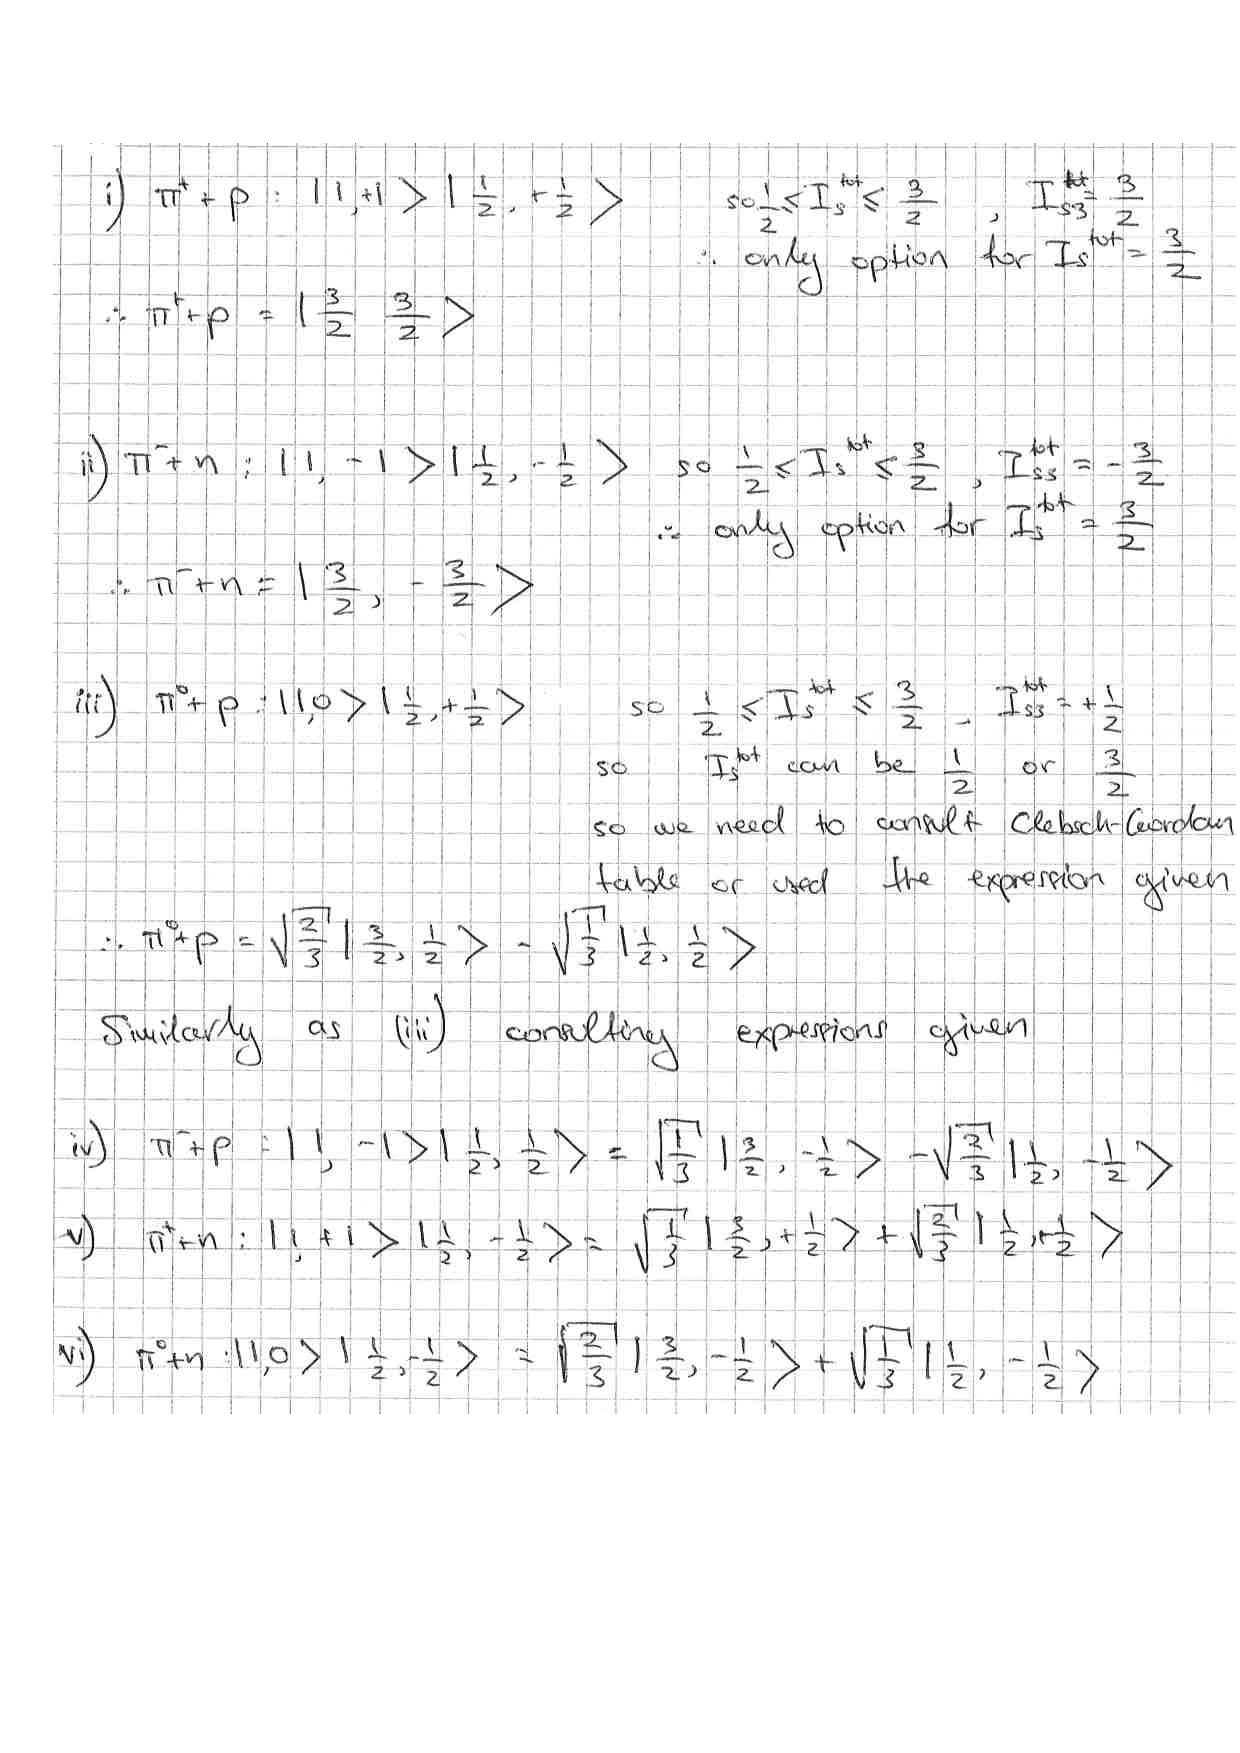
\includegraphics[width=0.98\textwidth]{problemsheets/fig/ans_ps2_strong_1.pdf}\\
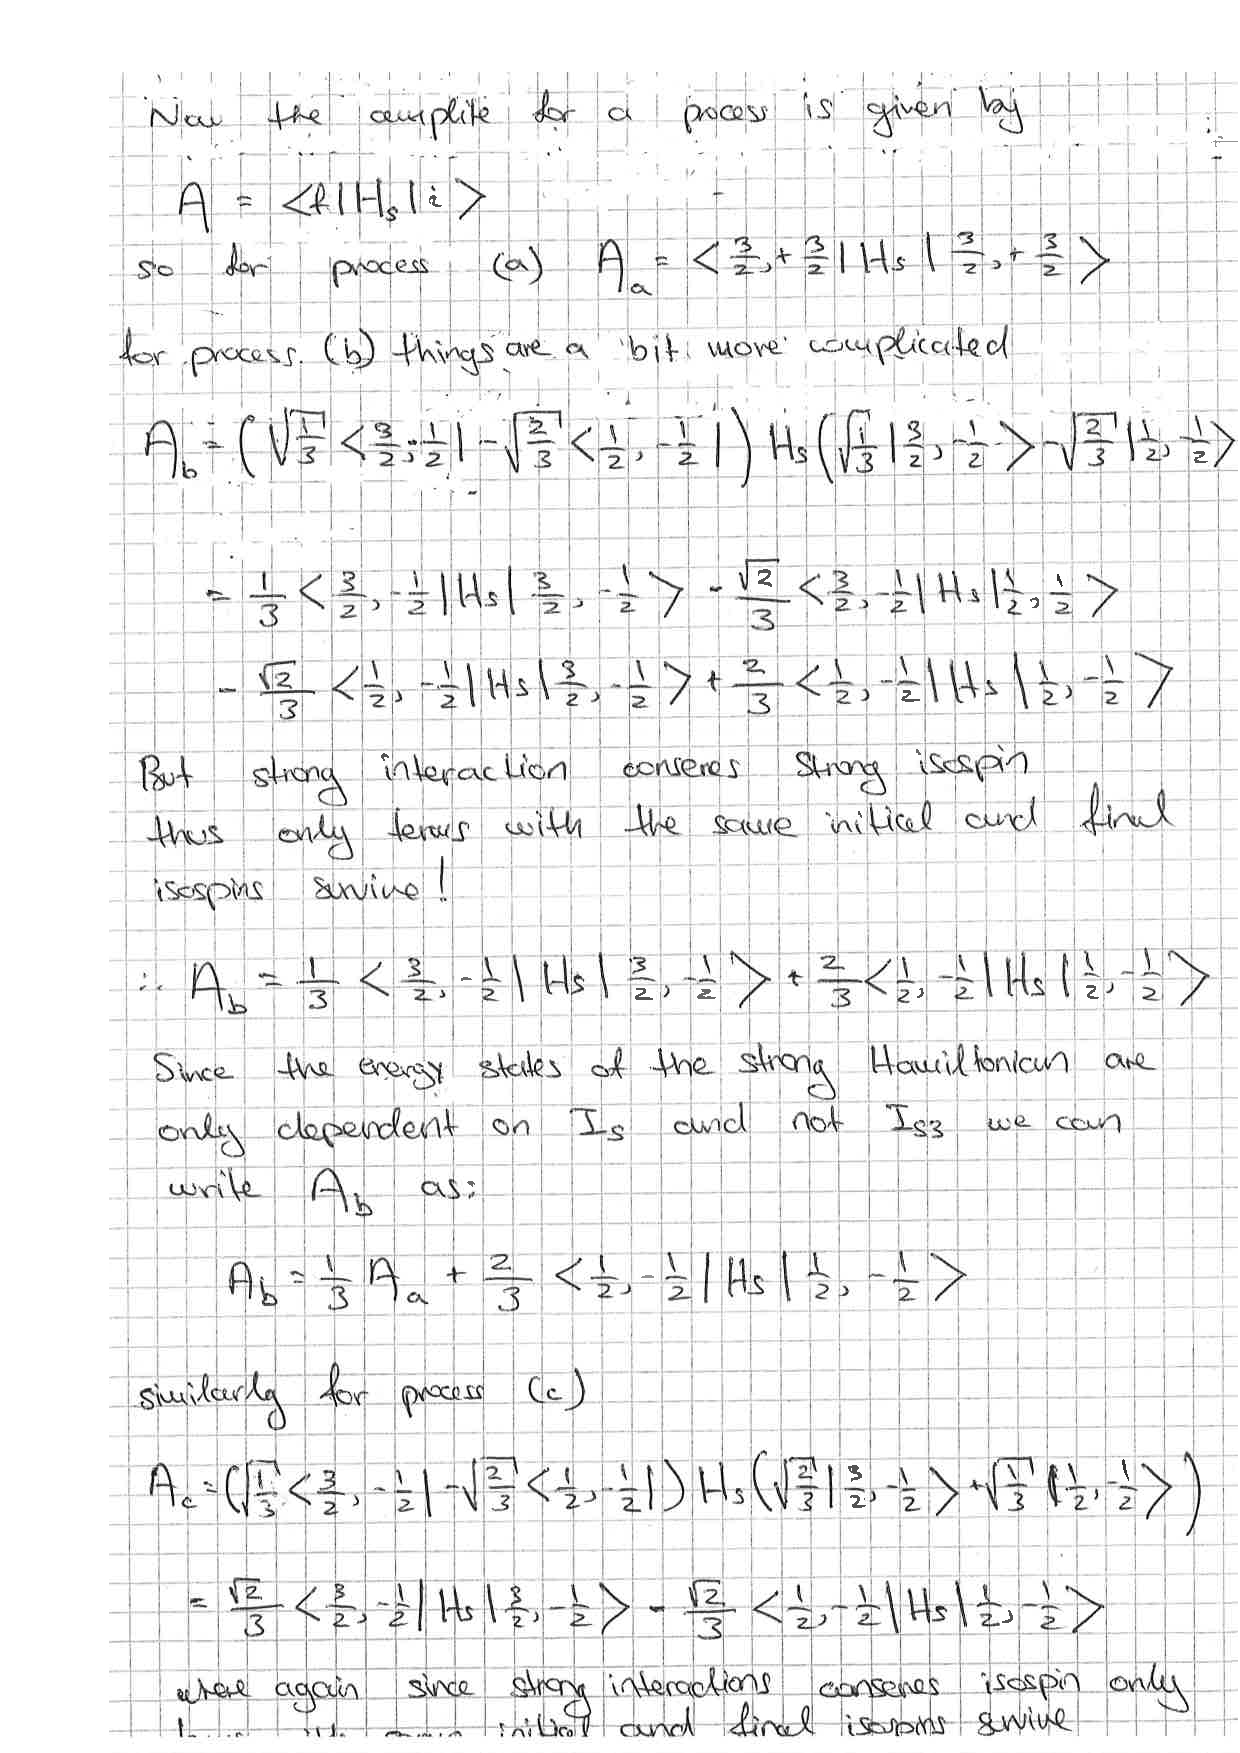
\includegraphics[width=0.98\textwidth]{problemsheets/fig/ans_ps2_strong_2.pdf}\\
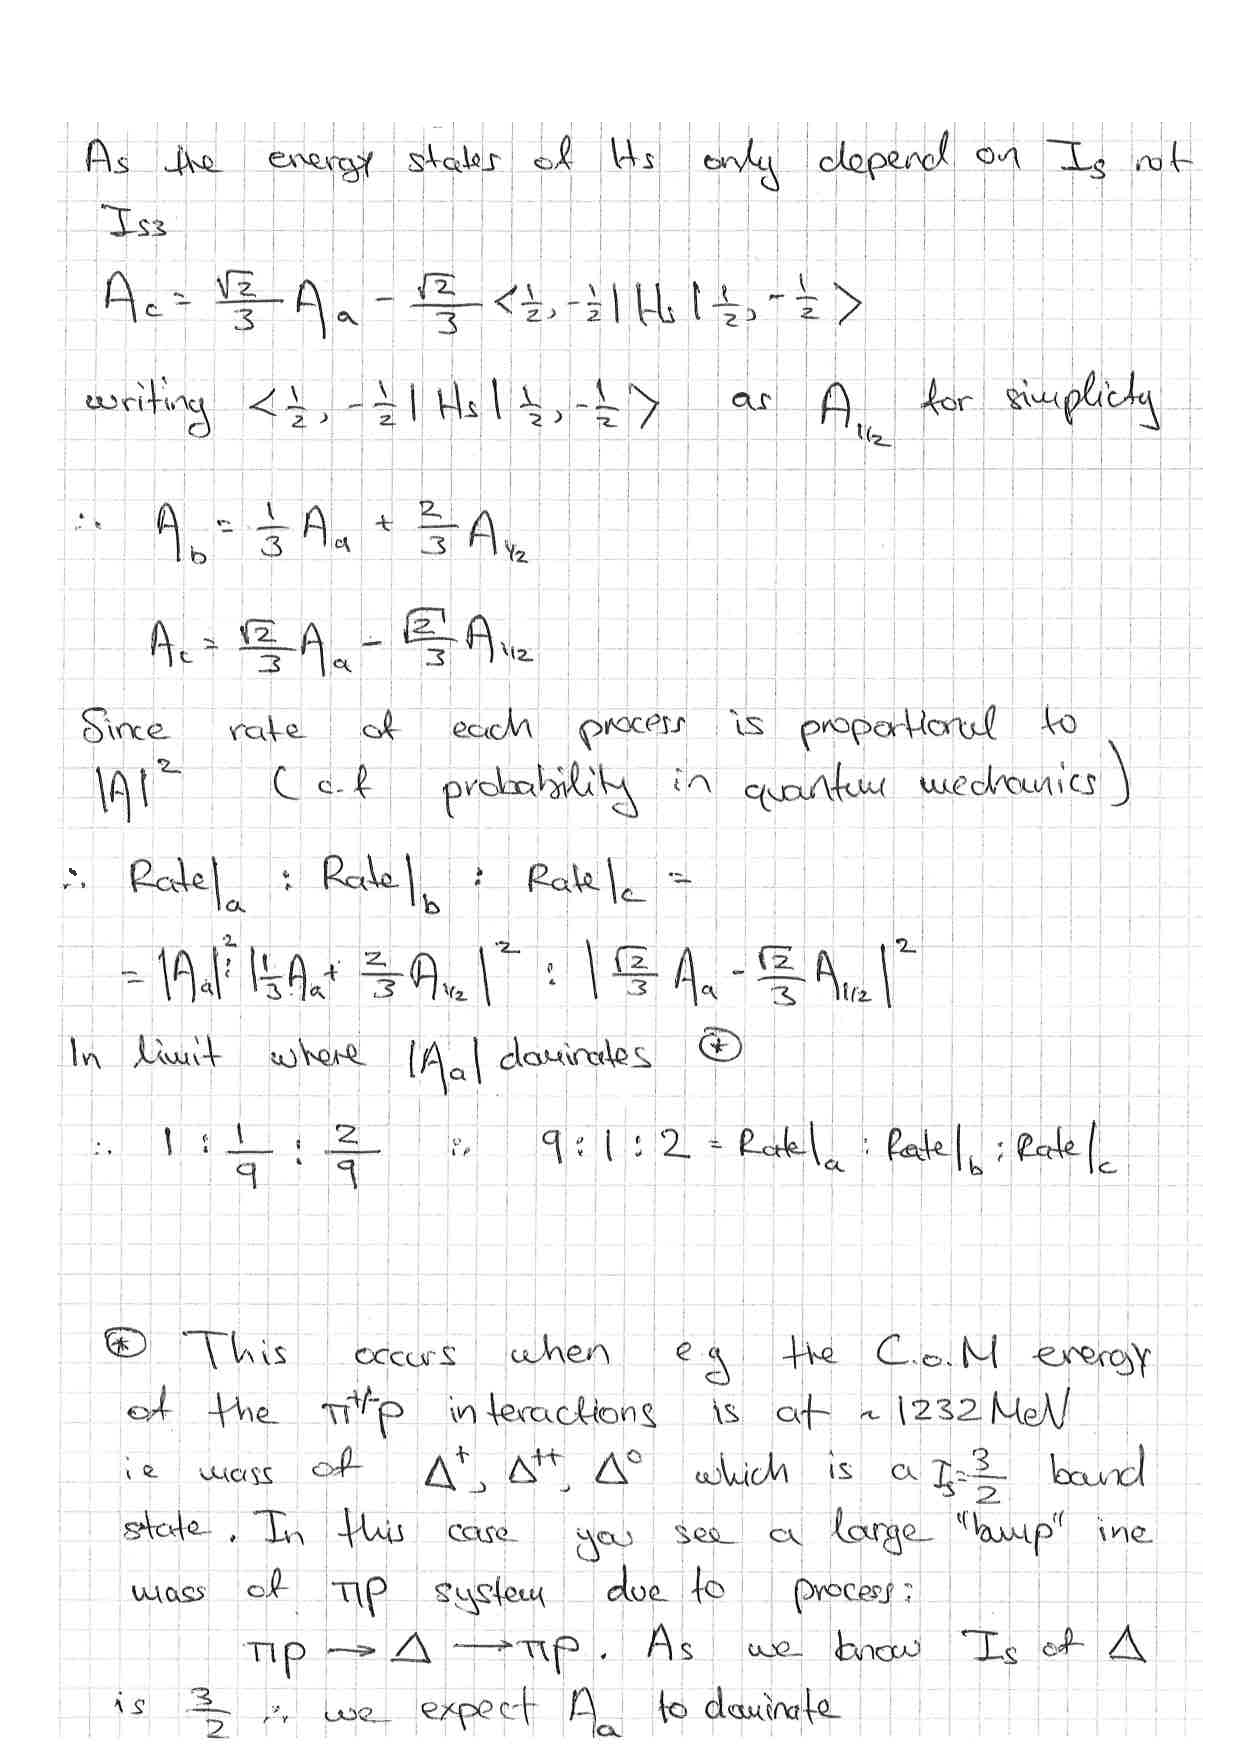
\includegraphics[width=0.98\textwidth]{problemsheets/fig/ans_ps2_strong_3.pdf}\\
}


\NewQuestion{Now coming back to the Dirac Equation and conservation of Total Angular Momentum}
\begin{enumerate}[(a)]
\item Show that the Dirac Hamiltonian
\[ \hat{H} = \gamma^{0}(\gamma^1\hat{p}_x+ \gamma^2\hat{p}_y + \gamma^3\hat{p}_z)+\gamma^{0}m, \]
can be written as
\[
\hat{H}=\mII{\underline{0}}{\vec{\sigma}\cdot\hat{\vec{p}}}{\vec{\sigma}\cdot\hat{\vec{p}}}{\underline{0}}+
\mII{m}{\underline{0}}{\underline{0}}{-m}
\]
where $\underline{0}$ denotes a $2\times2$ null-matrix.
You need to use the definition of the $\gamma$ matrices given in the notes.

\item Following this now show that

\[ [H,\hat{\Sigma}_x]=i\mII{\underline{0}}{\sigma_2\hat{p}_{z}-\sigma_3\hat{p}_{y}}{\sigma_2\hat{p}_{z}-\sigma_3\hat{p}_{y}}{\underline{0}} \]
\[ [H,\hat{\Sigma}_y]=i\mII{\underline{0}}{\sigma_3\hat{p}_{x}-\sigma_1\hat{p}_{z}}{\sigma_3\hat{p}_{x}-\sigma_1\hat{p}_{z}}{\underline{0}} \]
\[ [H,\hat{\Sigma}_z]=i\mII{\underline{0}}{\sigma_1\hat{p}_{y}-\sigma_2\hat{p}_{x}}{\sigma_1\hat{p}_{y}-\sigma_2\hat{p}_{x}}{\underline{0}} \]

where $\hat{\Sigma}_{x}=1/2\mII{\sigma_{1}}{\underline{0}}{\underline{0}}{\sigma_{1}}$, 
$\hat{\Sigma}_{y}=1/2\mII{\sigma_{2}}{\underline{0}}{\underline{0}}{\sigma_{2}}$, 
$\hat{\Sigma}_{z}=1/2\mII{\sigma_{3}}{\underline{0}}{\underline{0}}{\sigma_{3}}$. 

\item Now show the expressions you obtained in the previous question can be written as
\[
 [\hat{H},\hat{L}_x]  = -i\mII{\underline{0}}{\sigma_2\hat{p}_{z}-\sigma_3\hat{p}_{y}}{\sigma_2\hat{p}_{z}-\sigma_3\hat{p}_{y}}{\underline{0}}
\]                                                                                                                             
\[                                                                                                                             
  [\hat{H},\hat{L}_y] = -i\mII{\underline{0}}{\sigma_3\hat{p}_{x}-\sigma_1\hat{p}_{z}}{\sigma_3\hat{p}_{x}-\sigma_1\hat{p}_{z}}{\underline{0}}
\]                                                                                                                             
\[                                                                                                                             
 [\hat{H},\hat{L}_z]  = -i\mII{\underline{0}}{\sigma_1\hat{p}_{y}-\sigma_2\hat{p}_{x}}{\sigma_1\hat{p}_{y}-\sigma_2\hat{p}_{x}}{\underline{0}}
 \]

\item Therefore show that
  \[[H,\hat{\vec{J}}]=0\]
    where $\hat{\vec{J}}=\hat{\vec{L}}+\hat{\vec{\Sigma}}$
    
\end{enumerate}
\answerbox{
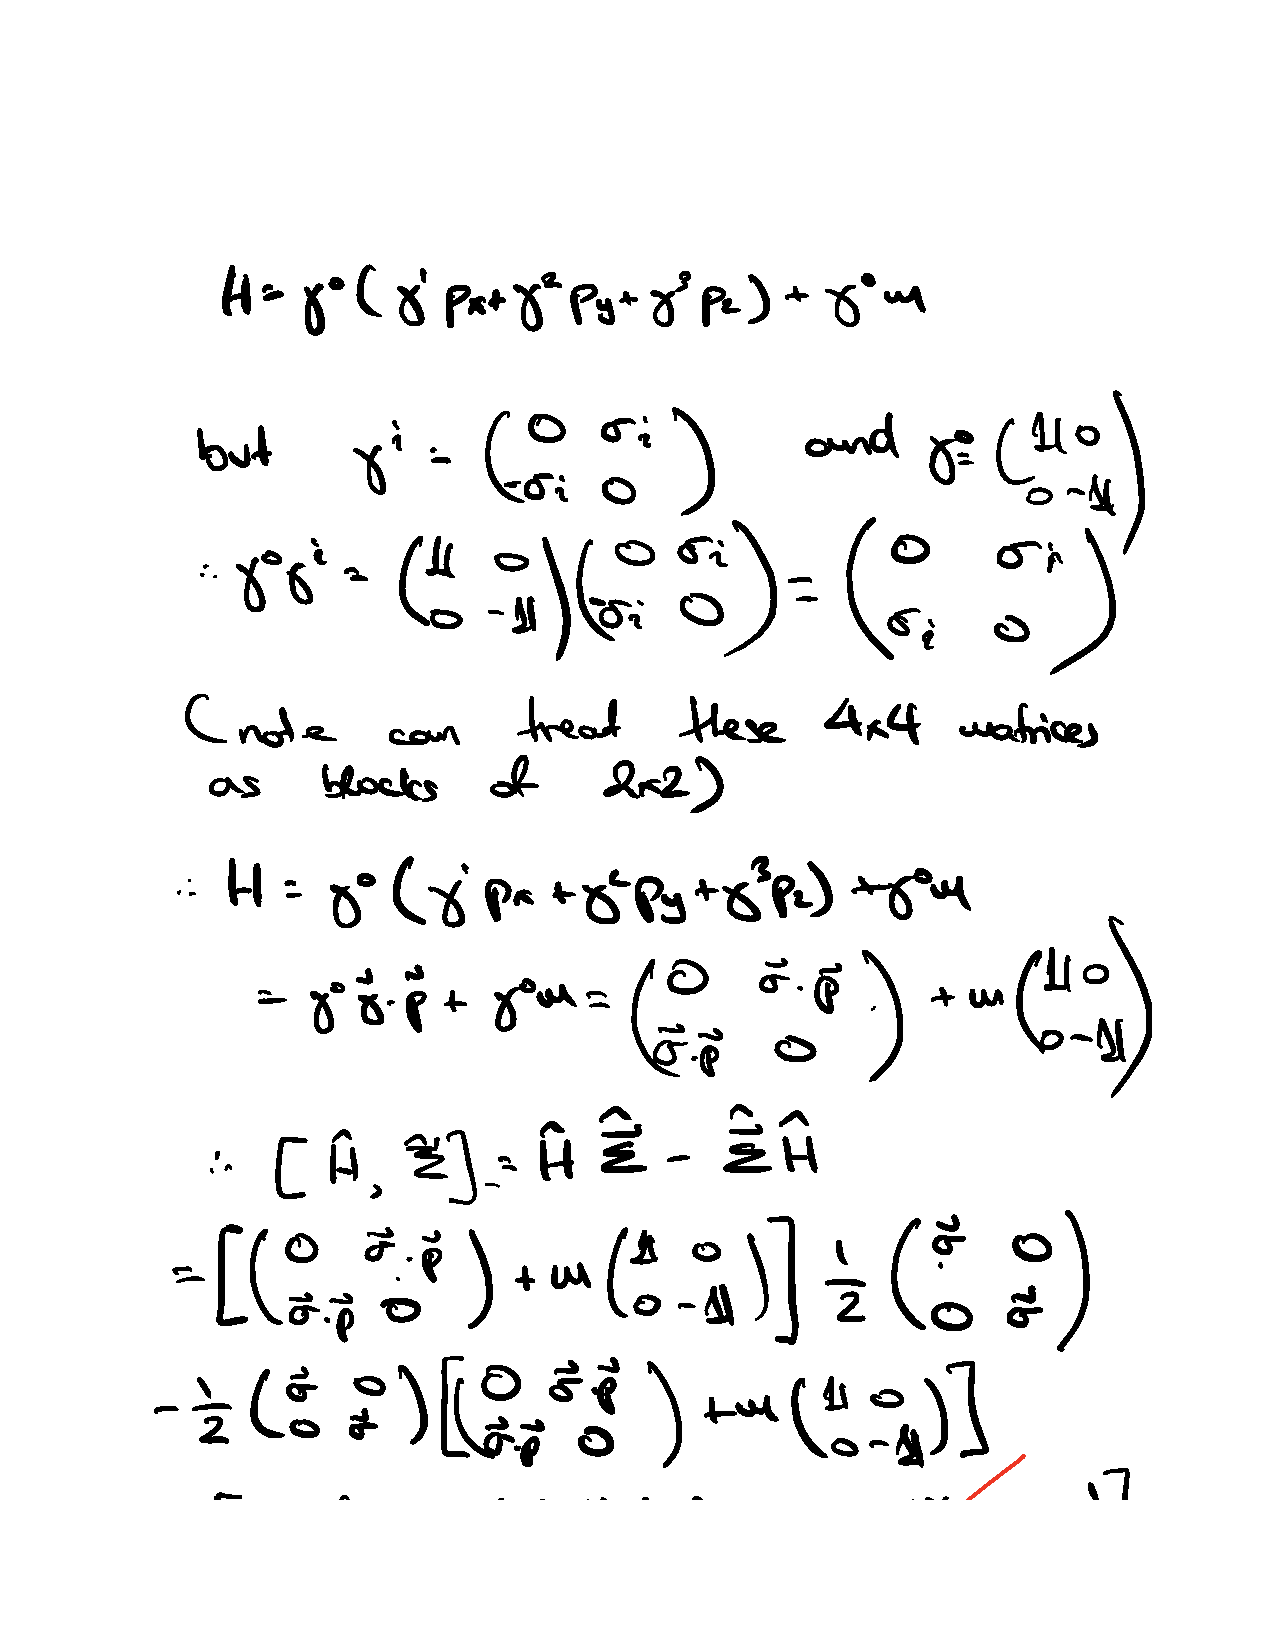
\includepdf[pages={1-},width=0.99\textwidth]{problemsheets/fig/ProblemSheet2Exercise5Answer.pdf}
}

\NewQuestion{This question is about the evidence of colour from the measurement of the so-called R-ratio. It accounts for the famous colour factor which was ommitted from the question of problem sheet 1}

A collider accelerates and collides beams of electrons and positrons a centre-of-mass energy $e^+e^-$ $\sqrt{s}=20$~GeV. Draw a Feynman diagram for the
  $e^+e^-\to\mu^+\mu^-$ process and the $e^+e^-\to q\overline{q}$
  process, where $q\overline{q}$ denotes any quark/anti-quark pair
  produced at this experiment. Clearly indicate on the diagrams the
  interaction strength at each vertex and the possible values of colour charge the quark and anti-quark can take.
  \answerbox{ Can choose to draw the $ee \to \mu\mu$ mediated by
    a photon with coupling proportional to $e\times e$. For the
    analogous $q\overline{q}$ final state, the coupling will be
    proportional to $e\times e_{q}$.}
 
 The experimenters intend to measure the fraction $R=\frac{\sigma(e^+e^-\to\mathrm{hadrons})}{\sigma(e^+e^-\to
    \mu^+\mu^-)}$. What value of R should they expect? Remember to consider what types of quarks can be produced at  $\sqrt{s}=20$~GeV. Do not forget to account for the colour factor.
    \answerbox{
    The collision energy means they can produce up to $b\overline{b}$
    pairs. You must remember the factor 3 colour factor.  Also note that $e_q = k\times e$ where $k=1/3$ (for $d,s,b$) or $2/3$ (for $u,c$). This means
    $R=3\times\sum\frac{e_{q}^{2}e^{2}}{e^{4}}=3\times(4/9+1/9+4/9+1/9+1/9)=33/9\sim3.67$
    }

\NewQuestion{Cosmic Radiation}
The predominant cause of cosmic radiation is protons that hit the earth's upper atmosphere. The resulting strong interactions produce lots of pions. A neutrino experiment on earth measures the ratio of the flux of muon neutrinos produced in the upper atmosphere (not distinguishing between \prt{\nu_{\mu}} and \prt{\overline{\nu}_{\mu}}) to the flux of
electron neutrinos (again, not distinguishing between \prt{\nu_{e}} and \prt{\overline{\nu}_{e}}). By considering the decay chain of the pions, what ratio should they expect? 
(Incidentally, what one would expect from these considerations is this is not what is observed. Look up "neutrino oscillations" or "Nobel Prize in Physics 2015" to find out why.)
\answerbox{
The process that creates the neutrinos is charged pion decay, which is predominantly \prt{\pi^+ \to \mu^+ \nu_{\mu}} (and the charged conjugate process, i.e. \prt{\pi^- \to \mu^- \overline{\nu}_{\mu}}), followed by the subsequent decay of the muon \prt{\mu^+ \to e^+ \nu_{e} \overline{\nu}_{\mu}} (and equivalently for the \prt{\mu^-}). So the expected ratio is 2.}

